\subsection{Essentials of probability theory and graph theory}
% 1 page

\subsubsection{Probability theory}
[chapter 2]

- probability: degree of belief that an event happens
- random variable: representing a set of events which are mutually exclusive, e.g. a die
- random variables have values
- probability distribution: assignment of real numbers to values of event, sum up to 1 $\Omega$
- joint distribution: combination of probability distribution of multiple random variables
- independence / conditional independence
- querying / expectation / variance: given certain events, how likely is a other event to occur

\subsubsection{Graph theory}

- nodes: in case of probabilistic models -> random variables
- edges: set of (ordered) pairs of nodes (can be directed or undirected), here we mainly refer to undirected edges
- subgraphs: subset of nodes including all edges amongst them if given in the original set of edges
- paths / trails: set of edges which connect two nodes -> if there is a path there is a dependency
- cycles / loops - set of edges with same starting and ending point, not using the same edge twice

\subsection{Introduction to undirected graphical model}
% 1 page

- nodes as random variables
- edges undirected representing dependencies
- example of undirected graphical model: with a good textual example (real life example)

As other graphical models like the Bayesian network the undirected graphical network consists of a set of nodes $V$ (also called vertices) and a set of edges between the nodes $E$, which is a set of tuples of exactly two nodes. The key difference to a Bayesian network is that those edges are not directed, in the meaning that the dependency between two nodes do not have a direction, as described in \cite{koller2009probabilistic}.

When the edges of a undirected graph represent random variables, it is called a undirected graphical model or also Markov network or Markov random field. The edges hereby represent a probabilistic dependency between the linked random variables, as \cite{kindermann1980markov} describes.

Figure \ref{fig:basic} shows a simple example of an graphical model (Markov network) with a set of four random variables $V=\{A,B,C,D\}$ and four probabilistic dependencies (edges): $E=\{(A,B),(B,C),(A,C),(C,D)\}$. In this example, the nodes could represent humans and the edges could represent a probabilistic presentation of how like it is, that two persons are relatives. Based on such a model the probability of how likely it is that all four persons are relatives could be calculated. To do so, it is necessary to parameterize the model.

\begin{figure}[htpb]
  \centering
  	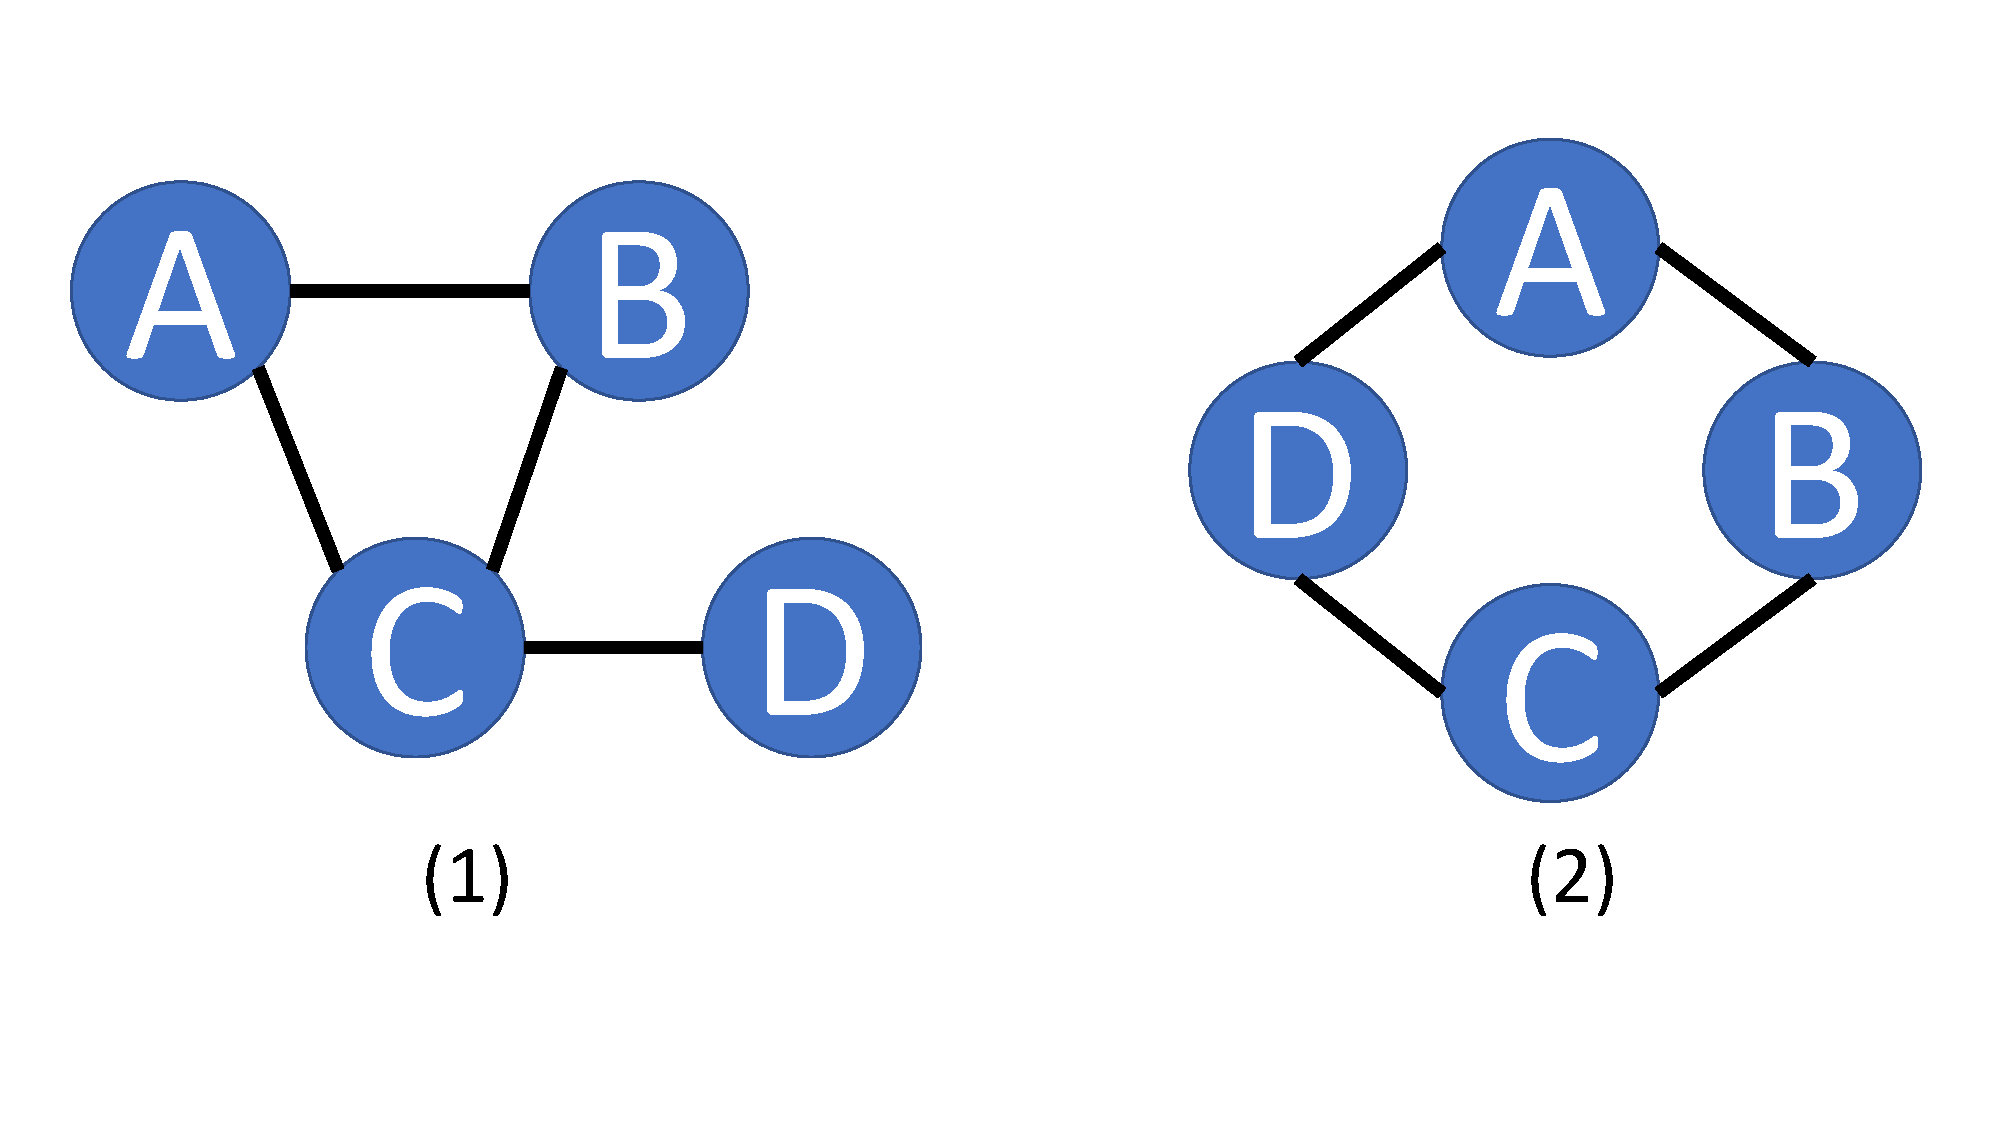
\includegraphics[scale=0.3]{img/basic.pdf} 
  \caption{Simple Undirected Graphical Model}
  \label{fig:basic}
\end{figure}

\subsection{Parameterization}
% 2 pages

- intro: probabilistic graphical model shall provide independences as well as the parameterization between the variables, so inference and learning is possible (ref to chapters down there)
- ref to cpd: as we will see in [ref to Bayesian network] conditional probability distributions are used, but this is not possible here cause the mutual dependency, but affinities of certain value combinations between dependent are expressed in real number (like compatibilities) -> in a factor
- factor: set of variables (cliques), do not have to sum up to 1
- factor-multiplication: multiply real numbers where values match up
- full joint distribution: unnormalized, normalized, inference by summing up probabilities -> REMEMBER Markov property, when a variable is cut of by given ones, it is independent
- table for a factor and table for a full joint distribution

In order to calculate probabilities on an undirected graphical model, the model needs to be parameterized in the first place. Such a parameterization is achieved by assigning factors to subsets of random variables of the graph. Each factor consists of parameters, which assign a real number to a certain combination of values the included random variables can adapt. If for example there is a factor over two binary random variables $A$ and $B$ the factor $\phi(A,B)$ would have four parameters for each combination of values of $A$ and $B$. Figure \ref{fig:param} shows such a factor and demonstrate the assignment of probabilities to each possible combination. If the assigned real numbers represent probabilities and not any kind of unnormalized score, they sum up to one, as shown in the figure.

\begin{figure}[htpb]
  \centering
  	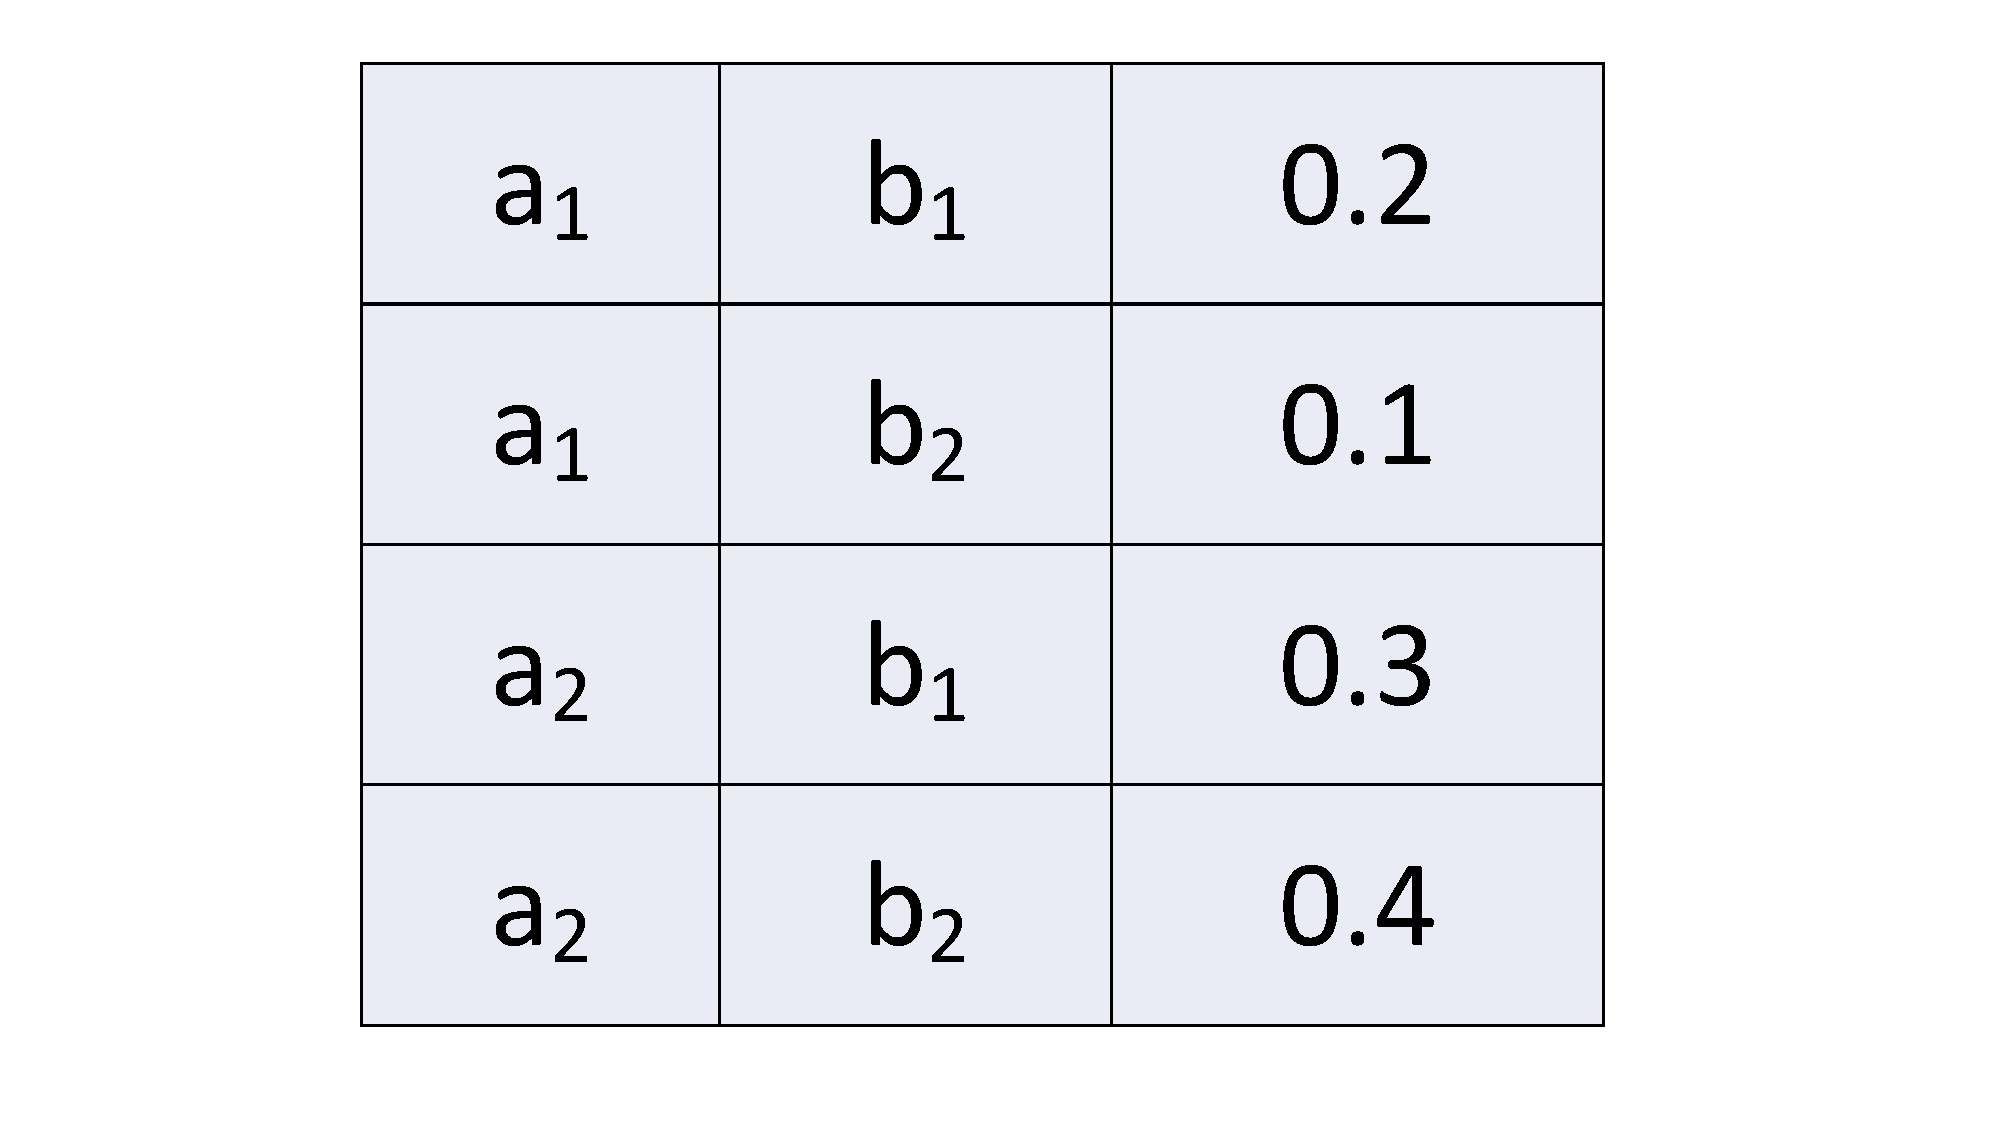
\includegraphics[scale=0.3]{img/param.pdf} 
  \caption{Factor of two binary linked random variables}
  \label{fig:param}
\end{figure}

TODO: refactor the factor product, refer to \cite{koller2009probabilistic} page 107 ff.

With this method all factors over two random variables, which are directly linked via an edge, can be expressed. Based on those factors we can calculate factors over larger subsets or the whole model. This is achieved by multiplying factors, which share at least one node, as for example $\phi(A,C)$ and $\phi(C,D)$ as shown in figure \ref{fig:basic}. When calculating the factor product, the probability of every parameter of the first factor is multiplied with the probability of the referring parameter of the second factor with respect to the shared random variable, such that for every different combination a parameter of the superior factor exists. If $A$, $C$ and $D$ for instance are binary random variables, the factor over those three nodes would have $2^3=8$ parameters, as shown in figure \ref{fig:parammult}.

\begin{figure}[htpb]
  \centering
  	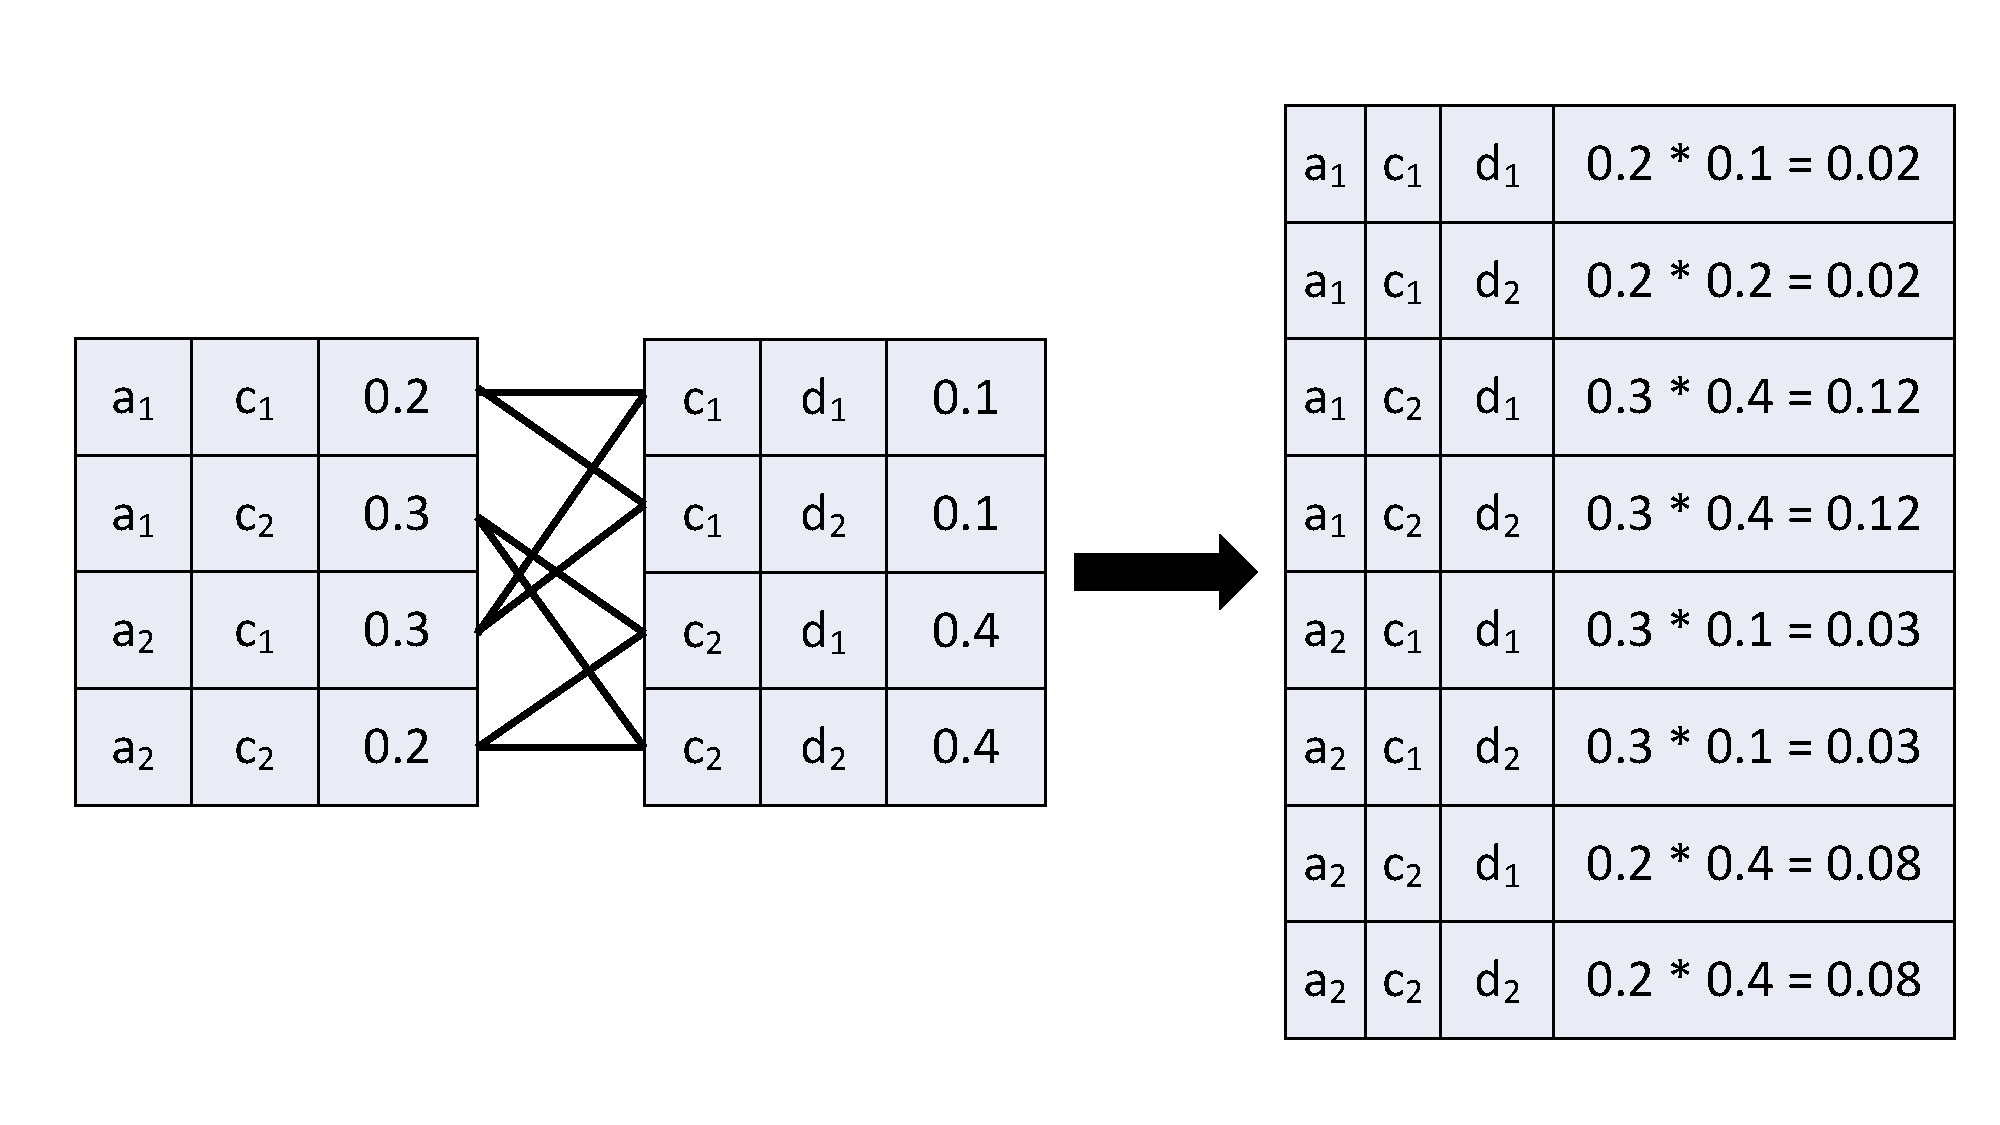
\includegraphics[scale=0.4]{img/parammult.pdf} 
  \caption{Factor multiplication of three binary random variables}
  \label{fig:parammult}
\end{figure}

Thus to compute a full joint distribution every single factor involved in this distribution needs to be taken into account. If the joint probability of the Markov network is strictly positive than this distribution is also considered a Gibbs distribution, as described in \cite{kindermann1980markov}.

\subsection{Independences in Markov networks}
% 0.5 page

- defined independences by Markov properties
- global
- local
- relationships

To be considered as a Markov network (or Markov random field) the random variables need to satisfy the following Markov properties with respect to the graph, as described in \cite{markov1957theory}:

\begin{enumerate}
\item Pairwise Markov property: Given all other random variables two non-adjacent (which means there is no edge between those two nodes) variables are conditionally independent.
\item Local Markov property: Given all its neighbors a random variable is conditionally independent of all other non-adjacent random variables.
\item Global Markov property: Any two subsets are conditionally independent if any path between them passes through a given third subset which is disjoint to those both.  
\end{enumerate}


\subsection{Inference on undirected models}
% 1 page

- Part II
- Brief: what can you do on undirected graphs, what is the specialty

\subsection{Learning on undirected models}
% 1 page

- Part III
- Brief: what can you do on undirected graphs, what is the specialty
